% Created 2020-05-06 mié 13:44
% Intended LaTeX compiler: pdflatex
\documentclass[a4paper, 12pt]{article}
\usepackage[utf8]{inputenc}
\usepackage[T1]{fontenc}
\usepackage{graphicx}
\usepackage{grffile}
\usepackage{longtable}
\usepackage{wrapfig}
\usepackage{rotating}
\usepackage[normalem]{ulem}
\usepackage{amsmath}
\usepackage{textcomp}
\usepackage{amssymb}
\usepackage{capt-of}
\usepackage{hyperref}
\usepackage{float, amsfonts, commath, mathtools}
\author{Tabaré Pérez}
\date{\today}
\title{Lecture 13 - 3: Introduction to Clustering}
\hypersetup{
 pdfauthor={Tabaré Pérez},
 pdftitle={Lecture 13 - 3: Introduction to Clustering},
 pdfkeywords={},
 pdfsubject={},
 pdfcreator={Emacs 26.3 (Org mode 9.3.6)}, 
 pdflang={English}}
\begin{document}

\maketitle
\textbf{Agenda}

\begin{itemize}
\item Understand the definition of \textbf{CLUSTERING}.
\begin{itemize}
\item Examples.
\end{itemize}
\item Understand \textbf{CLUSTERING COSTS} with different similarity measures.
\item Understand the \textbf{K-MEANS} algorithm.
\end{itemize}

Today we will start talking about unsupervised machine-learning algorithms. So
what you've seen so far in the class was focused on the supervised learning,
when you're provided training set, and traditionally your training set in
classification consisted of n training instances where each instance was
represented by a feature vector \(x^{(i)}\) and a label \(y^{(i)}\).

Classification:

\begin{equation}
S_n=\{(x^{(i)}, y^{(i)})|i=1 \ldots n\}
\end{equation}

And the goal of the algorithm was to learn the mapping from the feature vectors
to the corresponding label, and the training data was the main source for
learning such a mapping. So geometrically speaking, you were provided some
points, let's say some positive points and maybe some negative points, and you
were aiming to learn a separator that divides all the positive points from
negative points:

\begin{figure}[H]
\centering
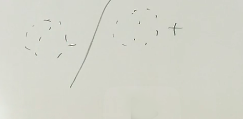
\includegraphics[width=0.5\textwidth]{./pic/04-03-fig-01.png}
\caption{\label{fig:org8c4e252}Supervised learning of positive and negative points}
\end{figure}

So all the algorithms that you've seen, like deep neural learning algorithm, for
instance, have many ways to accurately learn this mapping.

In unsupervised learning, we will still have a training set, to some extent, but
what we will not have are labels. So in this case, we are provided with just a
set of feature vectors, and you are trying to learn some meaningful structure
which would represent this set.

Clustering:

\begin{equation}
S_n=\{x^{(i)}|i=1 \ldots n\}
\end{equation}

And the type of algorithms we will cover today are called clustering algorithms.
So looking at this, you said when I was working on classification, it was clear
to me what was the goal of the learning. You had your label, correct? Now we
don't have any label. So in this particular instance, we may have just clouds of
our points, but we don't know any associated label y's.

Dibujo de nubes separadas sin separador lineal

So in this case, we can clearly see that even if we don't know the labels, there
is a very clear structure in our training data, and it will be meaningful for us
to automatically identify this structure.

So what we will do today, and this is our agenda for today:

We will study the question of how to automatically predict this meaningful
structure, and specifically we will talk about clustering algorithm, and what I
show you in the first part of the lecture is that you are already using
clustering in many situations in your life, and in many cases, the meaningful
structure is actually quite intuitive in the context of a specific application.

The second question  that we will address will relate to the fact, again, that
we don't have labels, and sometimes there are many possible ways to assign the
grouping to our points. So in order to determine which ones are good and which
ones are bad, we really need to know, what is the cost of the clustering? How do
I say if my clustering is good? And within this discussion we will talk about
different similarity measures, and we will translate our intuition into the
formulas which can be then utilized by the algorithm. So here we will complete
this part of the lecture by knowing exactly, given any partition of the points,
how to compute the quality of this partition.

And the third part of the lecture would be on K-means algorithm, which actually
can take any set of training point and find a partitioning to \(K\) clusters and
this is a very important algorithm. It is widely used, so it will be good for us
actually to learn it and to think how we can apply it to real problems.

So let me first start by talking about clustering from the application
perspective.

So one of the most common applications where we are using clustering is to help
us to visualize information and to improve our access to information.

Consider, for instance, Google News.

\begin{figure}[H]
\centering
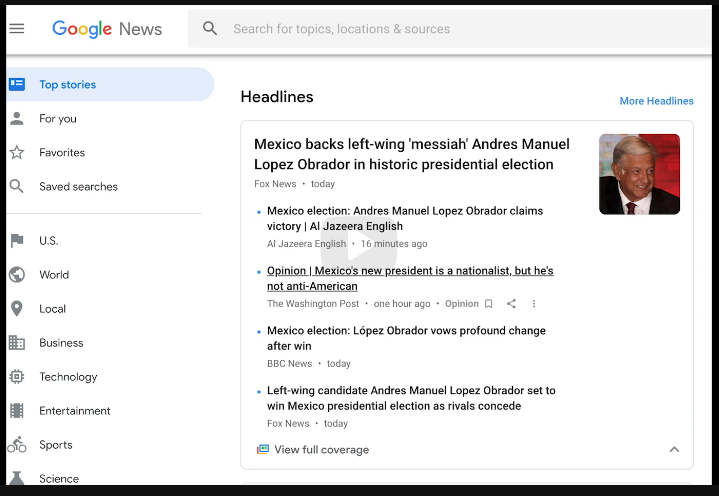
\includegraphics[width=0.5\textwidth]{./pic/intro-to-clustering-example-google-news.png}
\caption{\label{fig:orgc49eaaa}Google News example}
\end{figure}

So one of the most common examples where clustering is used is actually when you
are reading your news. So I read all my news with Google News.

And if you look at this interface, you should be able to find here an example of
both classification and clustering.

So let's start with classification because you're more familiar with it.

\begin{figure}[H]
\centering
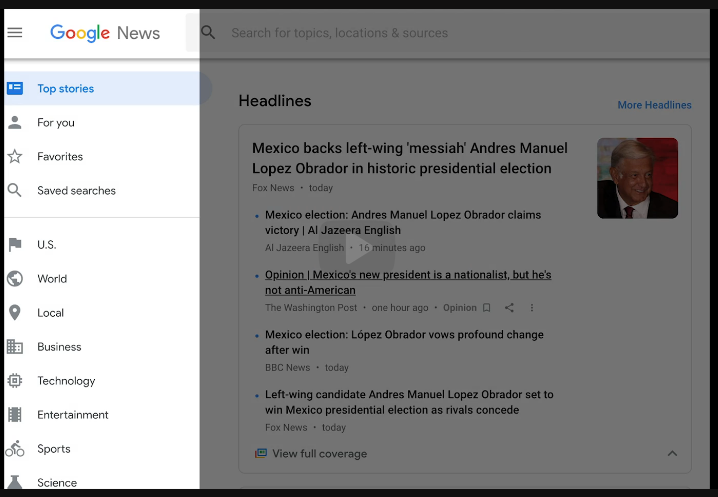
\includegraphics[width=0.5\textwidth]{./pic/google-news-classification.png}
\caption{\label{fig:org477c871}Google News Classification example}
\end{figure}

You can see that here every single piece of news is classified as belonging to
one of these categories, like US news or world news or local news and so on.

This was a classification because we had a limited set of tags, and we were
trying to classify every piece of news to one of these categories.

Now let's look at the sample of clustering.

\begin{figure}[H]
\centering
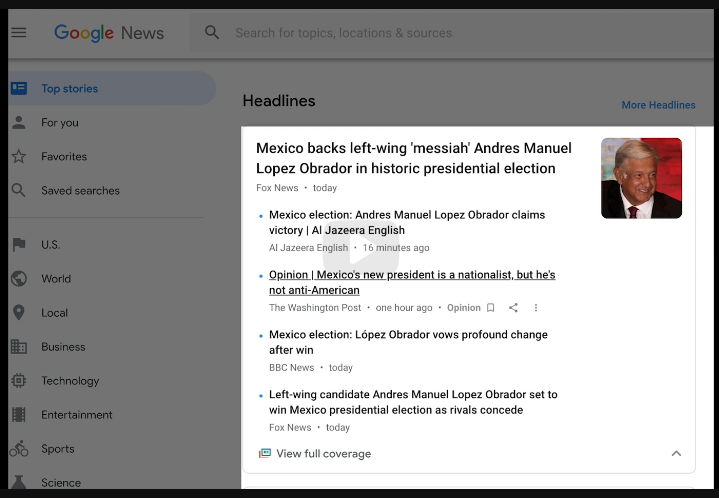
\includegraphics[width=0.5\textwidth]{./pic/google-news-clustering.png}
\caption{\label{fig:orgdbbdb87}Google News clustering}
\end{figure}

If you look now at this story about elections in Mexico, you would see that, in
addition to the top story, they also provide the whole set of stories that were
written above this event and similarly, we can see it above the second event and
this sports event. And instead of just showing one story about the event, Google
News clusters all the coverage about your current event and provides you access
to the whole group of stories about the single happening, and you can decide
which one you want to read.

So now let's think computationally. What do we need to do to build this kind of
clustering algorithm?

Obviously we don't have all the knowledge to implement it right now. We will
have it by the end of the lecture, but let's connect to what we already know.

So the first thing that we need to do in order for us to group the stories is we
need to have some computational mechanism to compare the two stories to decide
whether they're similar to each other or not.

So we can use a bag-of-words approach that we extensively discussed to represent
every story, and then we will use some measurements comparing the vectors that
represent the first story and the second story, for instance, cosine similarity.

So now for every pair of stories, you can say how close they are, and then you
need to have a clustering mechanism that actually enables you to effectively
group similar stories together, and that's exactly what enables us to produce
this type of representation, this type of clustering.

So whenever you're thinking about clustering, you can think to all these points
which are close to each other and, in this case, close in semantic space.

So, again, what were the three steps when I did the computation?

\begin{itemize}
\item I found out a representation of the stories, which was bag-of-words approach.
\item Then we need to decide how to compare each of these representations, in this
case vectors.
\item And the third one is to do the clustering algorithm itself.
\end{itemize}

Now let's move to another example.
\end{document}